\documentclass{article}
\usepackage[utf8]{inputenc}
\usepackage{graphicx}
\title{PS6_Tao}
\author{jiongliangtao }
\date{February 2019}

\begin{document}

\maketitle

\section{Question 3}
tweets.df <- twListToDF(tweets) 

Let tweets show as a dataframe. 

tweets.df2 <- gsub("http.*","",tweets.dfStext)
tweets.df2 <- gsub("https.*","",tweets.df2)
tweets.df2 <- gsub("#.*","",tweets.df2)
tweets.df2 <- gsub("@.*","",tweets.df2)
tweets.df2 <- gsub("RT","",tweets.df2)

Removing hashtag , urls and other special charactersR.

data <- data.frame(tweets = as.character(tweets.df2), 
                   stringsAsFactors = FALSE)
                   
Convert it to a data frame with string variables instead of a factor variable.

data <- data %>% 
    unnest-tokens(word, tweets)
    
Tokenize the tweets into words.

\section{Question 5}
The first graph shows people's manner to iphone xs max. It would be helpful for me to learn what manner people have with this topic. 

The second graph directly shows what words people use most in their tweets. It would be very helpful for me to see which word people use most in their tweets with this topic. 

The third graph shows the frequency of words that people use in their tweets.It would be helpful for me to see the frequency of the words because I can know what words people use most with this topic. 

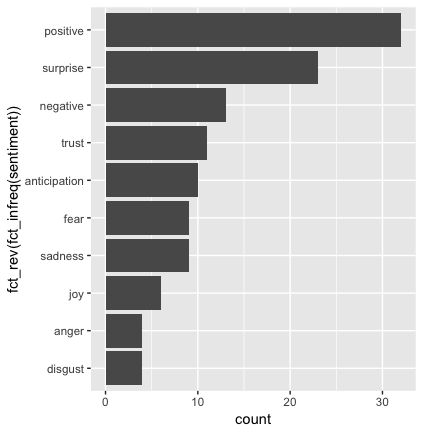
\includegraphics{PS6a_Tao.png}
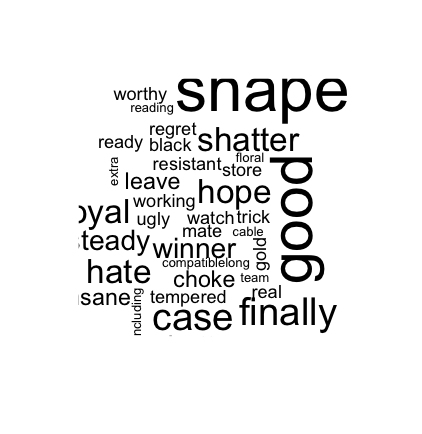
\includegraphics{PS6b_Tao.png}
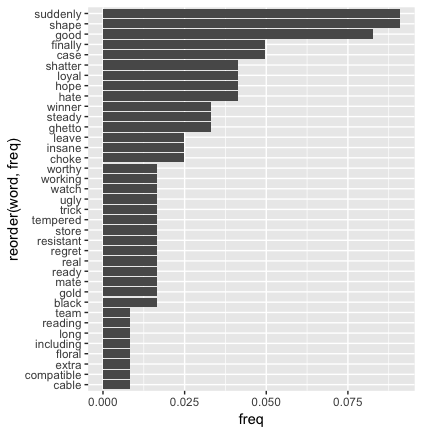
\includegraphics{PS6c_Tao.png}
\end{document}
